\documentclass{beamer}
%\usecolortheme{spruce}
\usetheme{bjeldbak}

\usepackage{tabularx}
\usepackage{amssymb}
\usepackage{stmaryrd}
\usepackage{proof}
\usepackage{bm}
\usepackage{booktabs}
\usepackage{multirow}
\usepackage{multicol}

\newcommand{\li}{\!\multimap\!}
\newcommand{\term}[1]{#1}
\newcommand{\mill}{ILL${}_{\multimap,\diamondsuit,\Box}$}
\newcommand{\proofspace}{\vphantom{()}}
\usepackage{tikz}
% Tikz configuration/libraries/macros
\usetikzlibrary{arrows,matrix,graphs,shapes,decorations,automata,backgrounds,petri,positioning,calc,decorations.pathmorphing,external,shapes.multipart}
\usetikzlibrary{decorations.pathreplacing}
\tikzstyle{underbrace style}=[decorate,decoration={brace,raise=7mm,amplitude=5pt,mirror}]
\tikzstyle{underbrace text style}=[below, pos=.5, yshift=-8mm]

\newcommand{\blocktitle}[1]{\normalsize\textcolor{pred}{#1}}
\newcommand{\posimpl}{\overset{+}{\multimap}}
\newcommand{\negimpl}{\overset{-}{\multimap}}
\newcommand{\posat}[1]{\overset{+}{#1\proofspace}}
\newcommand{\negat}[1]{\overset{-}{#1\proofspace}}
\hypersetup{
    colorlinks=true,
    linkcolor=black,
    filecolor=magenta,      
    urlcolor=cyan,
}


\begin{document}


\title[]{Neural Proof Nets}
\author{%
	\begin{tabularx}{0.7\textwidth}{@{}ccc@{}}
		Konstantinos							& \qquad 	Michael 							& 	\qquad Richard \\
		~Kogkalidis\inst{$\diamondsuit$} 	& \qquad 	~Moortgat\inst{$\diamondsuit$}	& 	\qquad ~Moot\inst{$\boxempty$}
	\end{tabularx}
	}
\institute{
	\inst{$\diamondsuit$} Utrecht Institute of Linguistics OTS, Utrecht University 
	\and 
	\inst{$\boxempty$} LIRMM, Universit\'{e} de Montpellier, CNRS }
\date[]{}

{%
\setbeamertemplate{headline}{}
\frame{\titlepage}
}

{%
   \begin{frame}
   \small
       \frametitle{Overview}       
       	\begin{block}{\blocktitle{tl;dr}}
       		A methodology to transcribe raw text to constructive proofs \& functional programs
		\end{block}
		\vfill
		
       \tableofcontents
   \end{frame}
}

\section{Theory}

\subsection{Typelogical grammars}

\begin{frame}{Typelogical grammars}
	\small
	\begin{block}{\blocktitle{Key points}}
	\begin{itemize}
		\item words are assigned \textit{formulas} of a constructive logic
		\item parsing is a formal deduction process:  parse $\equiv$ \textit{proof}
		\item Curry-Howard isomorphism: formula $\equiv$ \textit{type}, proof $\equiv$ \textit{program}
	\end{itemize}
	\end{block}
	
	\pause
	$\implies$ a syntactic parse becomes the instructions for an executable functional program.
\end{frame}

\begin{frame}{The logic}
	\small
	\begin{block}{\blocktitle{Modal implicational intuitionistic linear logic (ILL$_{\multimap,\diamondsuit,\Box}$)}}
	\mill\ contains types from the inductive set:
	\[
		\mathcal{T} := A \ | \ T_1 \li T_2 \ | \ \diamondsuit T \ | \ \Box T
	\]
	where 
	\begin{itemize}
		\item	$A$ an \textit{atomic} type, from a finite set $\mathcal{A}$
		\item $T_1 \li T_2$ a \textit{complex} type, denoting the transformation that consumes $T_1 
		\in \mathcal{T}$ to produce $T_2 \in \mathcal{T}$
		\item $\diamondsuit$, $\Box$ unary modalities
	\end{itemize}
	\end{block}
\end{frame}

\subsection{Type Logic: ILL${}_{\multimap, \diamondsuit, \Box}$}

\begin{frame}{ILL${}_{\multimap,\diamondsuit,\Box}$ and deep syntax}
	\small
	\alt<3>{	ILL${}_\multimap$ is a \textit{tecto-grammar} logic: it captures function-argument structures, ignoring word order and constituency structure.
	
	ILL${}_{\multimap,\diamondsuit,\Box}$, further captures \textit{dependency information} and constituency structure under a canonical word order.}{
		In our setup:
	\begin{itemize}
		\item	$\mathcal{A}$: a set of \textit{syntactic categories}, e.g. $\{n, np, s, pron, \dots \}$
		\item 	parameterized modalities $\diamondsuit^d$, $\Box^b$ where $d \in \mathcal{D}, b \in \mathcal{B}$:
		\vspace{-5pt}
		\begin{itemize}
		\item[$\triangleright$] 	$\mathcal{D}$: a set of \textit{complement markers}, e.g. $\{su, dobj, pobj, predc, \dots \}$
		\item[$\triangleright$] 	$\mathcal{B}$: a set of \textit{adjunct markers}, e.g. $\{mod, app, det, \dots \}$		
		\end{itemize}	
	\end{itemize}
	\vfill
	
	\pause
	A \textit{lexicon} $\mathcal{L}$ assigns types:
	\begin{itemize}
		\item 	from $\mathcal{A}$ to autonomous words, e.g. \\
				\footnotesize{blackbirds $:: np$, berries $:: np$}
		\item 	$\Box^b (T_1 \li T_2)$ to adjuncts, e.g.\\
				\footnotesize{the $:: \Box^{det}(np\li np)$}
		\item 	$\diamondsuit^d T_1 \li T_2$ to phrasal heads, e.g.\\
				\footnotesize{find $::  \diamondsuit^{predc}adj \li \diamondsuit^{dobj} np \li \diamondsuit^{su} np \li s$,\\
				that $:: \diamondsuit^{body}\left(\diamondsuit^{dobj}np \li s\right) \li \Box^{mod}\left(np\li np\right)$}
	\end{itemize}
	}
\end{frame}

\subsection{Proof Nets}
\begin{frame}{Proof nets for \mill}
	\small
	\begin{overlayarea}{1\textwidth}{0.4\textheight}
	\alt<5>{
		\begin{block}{\blocktitle{Traversal}}
		Traversal of a \mill\ proofnet induces a dependency-annotated $\lambda$-term, here:
		\[
			\term{\left(that\ \left(\lambda x^{dobj}. \left(eat\ x \right)\ blackbirds^{su} \right)^{body}\right)_{mod}
			\
			\left(the_{det}\ berries\right)}
		\]
		\end{block}
	}{
		\alt<4>{
			\begin{block}{\blocktitle{Proof net}}
			A proof net is a proof frame together with \textit{axiom links}, edges from positive to negative atoms.
			\end{block}
		}{
			\alt<2->{
				\begin{block}{\blocktitle{Type polarities}}
					Premise types $P_i$ are \textit{positive}, conclusion type $C$ is \textit{negative}.\\
					{\footnotesize
					\quad\textbf{Induction}:	\\
					\qquad If $A\li B$ positive, $A$ is negative, $B$ is positive.\\
					\qquad If $A\li B$ negative, $A$ is positive, $B$ is negative.
					}
				\end{block}
			}{
				\begin{block}{\blocktitle{Proof frame}}
				A proof frame is a judgement of the form $P_1, \dots P_n \vdash C$, with \textit{premises} $P_1, \dots P_n$ and \textit{conclusion} $C$ decomposed intro trees.
				\end{block}
			}
		}
	}
	\end{overlayarea}
	\vfill
	
	\scriptsize
	\begin{center}
	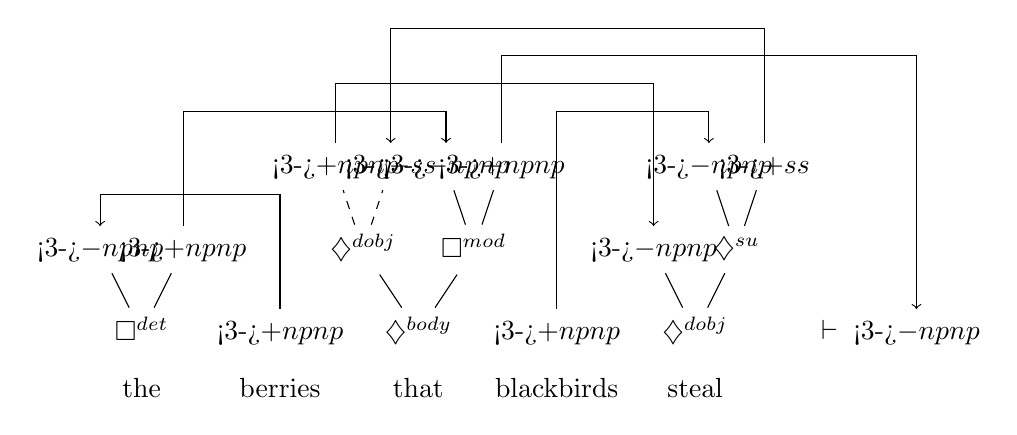
\begin{tikzpicture}
		% words
		\node (the)		at 	(0em, 0em)	{the};
		\node (berries)	at 	(5em, 0em)	{berries};
		\node (that)		at 	(10em, 0em)	{that};
		\node (birds) 	at 	(15em, 0em) 	{blackbirds};
		\node (steal)	at	(20em, 0em)	{steal};

		% undecorated trees
		\node (thedet)		at	(0em, 2em)		{$\Box^{det}\proofspace$};
		\node (thenp1)		at	(-1.5em, 5em)	{
			\alt<3->{$\negat{np}$}{$np\proofspace$}};
		\node (thenp2)		at	(1.5em, 5em)		{
			\alt<3->{$\posat{np}$}{$np\proofspace$}};
		\node (berriesnp)	at 	(5em, 2em)		{
			\alt<3->{$\posat{np}$}{$np\proofspace$}};
		\node (thatbody)		at	(10em, 2em)		{$\diamondsuit^{body}\proofspace$};
		\node (thatobj)		at	(8em, 5em)	{$\diamondsuit^{dobj}\proofspace$};
		\node (thatobjnp)	at	(7em, 8em)		{
			\alt<3->{$\posat{np}$}{$np\proofspace$}};
		\node (thats)		at	(9em, 8em)		{
			\alt<3->{$\negat{s}$}{$s\proofspace$}};
		\node (thatmod)		at	(12em, 5em)	{$\Box^{mod}\proofspace$};
		\node (thatmodnp1)	at	(11em, 8em)	{
			\alt<3->{$\negat{np}$}{$np\proofspace$}};
		\node (thatmodnp2)	at	(13em, 8em)	{
			\alt<3->{$\posat{np}$}{$np\proofspace$}};
		\node (birdsnp)		at	(15em, 2em)		{
			\alt<3->{$\posat{np}$}{$np\proofspace$}};
		\node (stealobj)		at	(20em, 2em)		{$\diamondsuit^{dobj}\proofspace$};
		\node (stealobjnp)	at	(18.5em, 5em)	{
			\alt<3->{$\negat{np}$}{$np\proofspace$}};
		\node (stealsu)		at	(21.5em, 5em)	{$\diamondsuit^{su}\proofspace$};
		\node (stealsunp)	at  (20.5em, 8em)	{
			\alt<3->{$\negat{np}$}{$np\proofspace$}};
		\node (steals)		at 	(22.5em, 8em)	{
			\alt<3->{$\posat{s}$}{$s\proofspace$}};
		\node (vdash)		at 	(25em, 2em)		{$\vdash\proofspace$};
		\node (finalnp)		at 	(28em, 2em)		{
			\alt<3->{$\negat{np}$}{$np\proofspace$}};

		% internal links
		\draw (thedet)   -- (thenp1);
		\draw (thedet)   -- (thenp2);
		\draw (stealobj) -- (stealobjnp);
		\draw (stealobj) -- (stealsu);
		\draw (stealsu)  -- (stealsunp);
		\draw (stealsu)  -- (steals);
		\draw (thatbody) -- (thatobj);
		\draw (thatobj)   edge[dashed] (thatobjnp);
		\draw (thatobj)   edge[dashed] (thats);
		\draw (thatmod)  -- (thatmodnp1);
		\draw (thatmod)  -- (thatmodnp2);
		\draw (thatbody) -- (thatmod);
		
		% axiom links
		\visible<4->{
		\draw[->] (berriesnp) -- ($(berriesnp) + (0em, 5em)$) -| (thenp1);
		\draw[->] (thenp2) -- ($(thenp2) + (0em, 5em)$) -| (thatmodnp1);
		\draw[->] (thatobjnp) -- ($(thatobjnp) + (0em,3em)$) -| (stealobjnp);
		\draw[<-] (thats) -- ($(thats) + (0em, 5em)$) -| (steals);
		\draw[->] (thatmodnp2) -- ($(thatmodnp2) + (0em, 4em)$) -| (finalnp);
		\draw[->] (birdsnp) -- ($(birdsnp) + (0em, 8em)$) -| (stealsunp);
		}
	\end{tikzpicture}
	\end{center}
\end{frame}

\section{Practice}
\subsection{Data}
\begin{frame}{Dataset}
	\small
	We use the \AE thel dataset: \hfill{\footnotesize(\href{https://arxiv.org/abs/1912.12635}{abs/1912.12635})}
	\begin{itemize}
		\item 72\,192 dutch sentences as \mill\ proofs
		\item 913\,404 typed words
		\item 5\,747 unique types, made of
		\begin{itemize}
			\item[$\triangleright$] 32 syntactic categories ($\mathcal{A}$)
			\item[$\triangleright$] 22 dependency labels ($\mathcal{D}\cup\mathcal{B}$)
		\end{itemize}
	\end{itemize}
\end{frame}

\subsection{Supertagging}
\begin{frame}{Supertagging}
	\small
	\alt<3->{
		\begin{block}{\blocktitle{seq2seq supertagging}}
		proof frames decoded using output vocabulary $\mathcal{A}\cup\mathcal{D}\cup\mathcal{B}\cup\left\{\#\right\}$
		\begin{itemize}
			\item no hard-coded vocabulary \hfill{(\href{https://arxiv.org/abs/1905.13418}{abs/1905/13418})}
			\item reusable representations for primitive symbols
		\end{itemize}
		\end{block}	
		
		\begin{block}{\blocktitle{implementation}}
			BERT-encoder, Transformer-decoder, symbols embedded in $\mathbb{C}$
		\end{block}
	}{
	We flatten type trees to prefix notation:
	
	\begin{center}
	{\footnotesize
	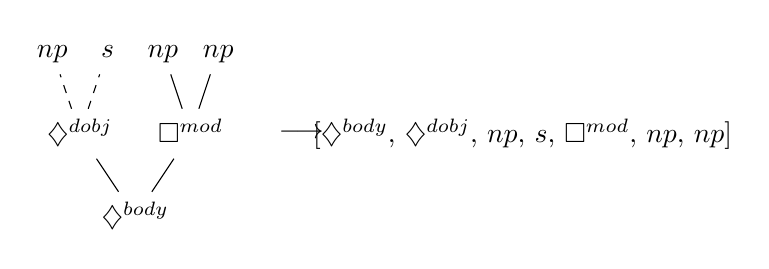
\begin{tikzpicture}
	\node (thatbody)			at	(10em, 2em)	{$\diamondsuit^{body}\proofspace$};
		\node (thatobj)		at	(8em, 5em)	{$\diamondsuit^{dobj}\proofspace$};
		\node (thatobjnp)	at	(7em, 8em)	{$np\proofspace$};
		\node (thats)		at	(9em, 8em)	{$s\proofspace$};
		\node (thatmod)		at	(12em, 5em)	{$\Box^{mod}\proofspace$};
		\node (thatmodnp1)	at	(11em, 8em)	{$np\proofspace$};
		\node (thatmodnp2)	at	(13em, 8em)	{$np\proofspace$};
		\draw (thatbody) -- (thatobj);
		\draw (thatobj)   edge[dashed] (thatobjnp);
		\draw (thatobj)   edge[dashed] (thats);
		\draw (thatmod)  -- (thatmodnp1);
		\draw (thatmod)  -- (thatmodnp2);
		\draw (thatbody) -- (thatmod);
		\node (convert) 		at 	(16em, 5em)	{$\longrightarrow$};
		\node (polish)		at 	(24em, 5em)  
		{[$\diamondsuit^{body}$, $\diamondsuit^{dobj}$, $np$, $s$, $\Box^{mod}$, $np$, $np$]};
	\end{tikzpicture}
	}
	\end{center}

	\pause
	a proof frame is then the concatenation of flattened types:
	\footnotesize
	\[
		\hspace{-10pt}
		\left[
			\underbrace{\Box^{mod},\ np,\ np,\ }_{\text{the}}
			\#,\
			\underbrace{np,\ }_{\text{berries}}
			\#,\
			\underbrace{\diamondsuit^{body},\ {\diamondsuit}^{dobj},\ np,\ s,\ \Box^{mod},\ np,\ np,\ }_{\text{that}} 
			\#,\
			\underbrace{\ np,\ }_{\text{blackbirds}}
			\dots
		\right]
	\]
	}
\end{frame}

\subsection{Parsing as permutation}

\begin{frame}{Parsing as permutation}
	\alt<4->{
			\begin{block}{\blocktitle{Obtaining permutation matrices}}
				\begin{enumerate}
					\item parse decoded types to obtain polarity information
					\item contextualize atoms \textbackslash w sentence \hfill{\footnotesize (bi-modal encoder)}
					\item for each atomic type $A$:
					\vspace{-3pt}
					\begin{itemize}
					\footnotesize
						\item[$\triangleright$] index \& extract positive and negative vectors $A_p, A_n$
						\item[$\triangleright$] compute their pair-wise matching as $A_pA^\top_n$
						\item[$\triangleright$] normalize to bistochasticity by iterating the \textit{Sinkhorn operator}*
					\end{itemize}
				\end{enumerate}
				\end{block}
			\footnotesize
			(*) a 2-dimensional, assignment-preserving softmax:
			\begin{itemize}
				\item structural correctness with no explicit structure
				\item easy training with negative log-likelihood
				\item sentence- and batch-wide parallelism
			\end{itemize}
	}{
		% pnet and tables
		\scriptsize
		\begin{center}
		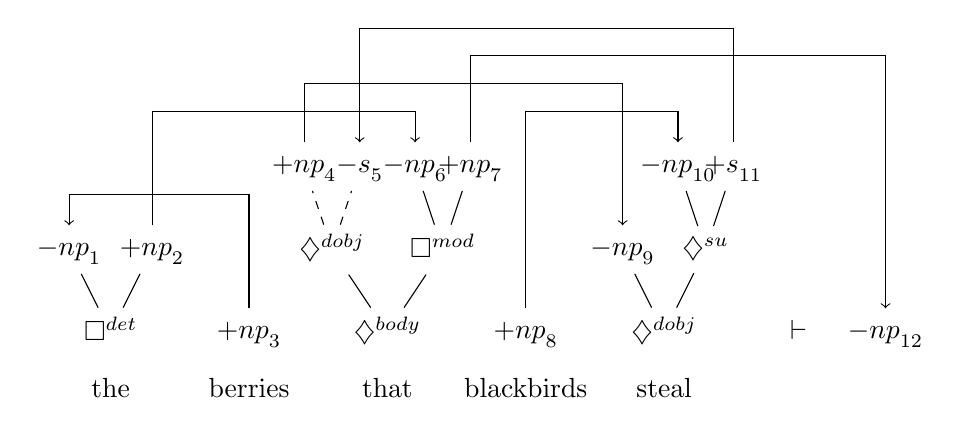
\begin{tikzpicture}
			% words
			\node (the)		at 	(0em, 0em)	{the};
			\node (berries)	at 	(5em, 0em)	{berries};
			\node (that)		at 	(10em, 0em)	{that};
			\node (birds) 	at 	(15em, 0em) 	{blackbirds};
			\node (steal)	at	(20em, 0em)	{steal};
	
			% undecorated trees
			\node (thedet)		at	(0em, 2em)		{$\Box^{det}\proofspace$};
			\node (thenp1)		at	(-1.5em, 5em)	{$\negat{np}_1$};
			\node (thenp2)		at	(1.5em, 5em)		{$\posat{np}_2$};
			\node (berriesnp)	at 	(5em, 2em)		{$\posat{np}_3$};
			\node (thatbody)		at	(10em, 2em)		{$\diamondsuit^{body}\proofspace$};
			\node (thatobj)		at	(8em, 5em)		{$\diamondsuit^{dobj}\proofspace$};
			\node (thatobjnp)	at	(7em, 8em)		{$\posat{np}_4$};
			\node (thats)		at	(9em, 8em)		{$\negat{s}_5$};
			\node (thatmod)		at	(12em, 5em)		{$\Box^{mod}\proofspace$};
			\node (thatmodnp1)	at	(11em, 8em)		{$\negat{np}_6$};
			\node (thatmodnp2)	at	(13em, 8em)		{$\posat{np}_7$};
			\node (birdsnp)		at	(15em, 2em)		{$\posat{np}_8$};
			\node (stealobj)		at	(20em, 2em)		{$\diamondsuit^{dobj}\proofspace$};
			\node (stealobjnp)	at	(18.5em, 5em)	{$\negat{np}_9$};
			\node (stealsu)		at	(21.5em, 5em)	{$\diamondsuit^{su}\proofspace$};
			\node (stealsunp)	at  (20.5em, 8em)	{$\negat{np}_{10}$};
			\node (steals)		at 	(22.5em, 8em)	{$\posat{s}_{11}$};
			\node (vdash)		at 	(25em, 2em)		{$\vdash\proofspace$};
			\node (finalnp)		at 	(28em, 2em)		{$\negat{np}_{12}$};
	
			% internal links
			\draw (thedet)   -- (thenp1);
			\draw (thedet)   -- (thenp2);
			\draw (stealobj) -- (stealobjnp);
			\draw (stealobj) -- (stealsu);
			\draw (stealsu)  -- (stealsunp);
			\draw (stealsu)  -- (steals);
			\draw (thatbody) -- (thatobj);
			\draw (thatobj)   edge[dashed] (thatobjnp);
			\draw (thatobj)   edge[dashed] (thats);
			\draw (thatmod)  -- (thatmodnp1);
			\draw (thatmod)  -- (thatmodnp2);
			\draw (thatbody) -- (thatmod);
			
			% axiom links
			\draw[->] (berriesnp) -- ($(berriesnp) + (0em, 5em)$) -| (thenp1);
			\draw[->] (thenp2) -- ($(thenp2) + (0em, 5em)$) -| (thatmodnp1);
			\draw[->] (thatobjnp) -- ($(thatobjnp) + (0em,3em)$) -| (stealobjnp);
			\draw[<-] (thats) -- ($(thats) + (0em, 5em)$) -| (steals);
			\draw[->] (thatmodnp2) -- ($(thatmodnp2) + (0em, 4em)$) -| (finalnp);
			\draw[->] (birdsnp) -- ($(birdsnp) + (0em, 8em)$) -| (stealsunp);
		\end{tikzpicture}
		\end{center}	
		\vfill
	
		\visible<2->{
		\begin{minipage}[c]{0.5\textwidth}
		\hspace{50pt}
		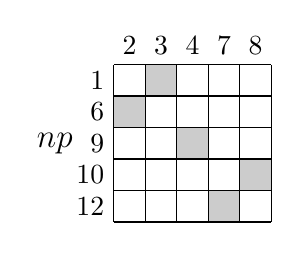
\begin{tikzpicture}[scale=.4]
		% matches
		\fill[gray!40] (1, 4) rectangle +(1,1);
		\fill[gray!40] (0, 3) rectangle +(1,1);
		\fill[gray!40] (2, 2) rectangle +(1,1);
		\fill[gray!40] (4, 1) rectangle +(1,1);
		\fill[gray!40] (3, 0) rectangle +(1,1);
		\node [above] at (0.5, 5)	{2};
		\node [above] at (1.5, 5)	{3};
		\node [above] at (2.5, 5)	{4};
		\node [above] at (3.5, 5)	{7};
		\node [above] at (4.5, 5)	{8}; 
		\node [left] at (0, 4.5)		{1};
		\node [left] at (0, 3.5)		{6};
		\node [left] at (0, 2.5)		{9};
		\node [left] at (0, 1.5)		{10};    
	    \node [left] at (0,0.5) 		{12};
	    \node [left] at (-1,2.5)	 	{\large $np$};
	    \draw (0,0) grid (5,5);
	    \end{tikzpicture}
		\end{minipage}%
		\begin{minipage}[c]{0.5\textwidth}
		\hspace{20pt}
	    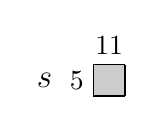
\begin{tikzpicture}[scale=0.4]
	    % matches
	    \fill[gray!40] (0,0) rectangle +(1,1);
	    \draw (0, 0) grid (1,1);
		\node[left] at (0, 0.5) {5};
		\node[above] at (0.5, 1) {11};
	    \node [left] at (-1,0.5)	 	{\large $s$};
	    \end{tikzpicture}
		\end{minipage}
		}
	}
\end{frame}

\begin{frame}{Table with numbers}
	\footnotesize
	
	\begin{center}
	\renewcommand{\arraystretch}{1.1}
	\begin{tabularx}{0.7\textwidth}{@{}c|ccc@{}}
	\multirow{2}{*}{metric} 				& 	baseline 	 & \multicolumn{2}{c}{our model}	\\
										& 	(alpino)		& greedy		&  5 beams			\\
	\toprule
	type accuracy						&	56.2			& 85.5		&	93.2				\\
	frame correct						&	46.6			& 57.6		&	69.6				\\
	ILL${}_{\li}$ correct 				&	45.7			& 60.0		& 	69.1				\\
	\mill\ correct *				 		&   30.4			& 56.9		&  	67.1				\\
	\hfill \textbackslash w type oracle 	& 	-			& 87.4		& 	-
	\end{tabularx}
	\end{center}\vfill

	(*) in practical terms:\\
	of sentences correctly converted to \textit{well-typed programs} \\
	\hfill (tagged, parsed and dependency-annotated)

	\vfill
	paper (preprint): \hfill \href{https://arxiv.org/abs/2009.12702}{abs/2009.12702}\\
	code, model \& data publicly available: \\	
	\hfill \url{https://github.com/konstantinosKokos/neural-proof-nets}
\end{frame}


\end{document}
